% Document type and package imports.
\documentclass[a4paper, 11pt]{article}
\usepackage[utf8]{inputenc}
\usepackage[T1]{fontenc}
\usepackage[french]{babel}
\usepackage{charter}
\usepackage[top = 2cm, bottom = 2cm, left = 1cm, right = 1cm]{geometry}
\usepackage{setspace}
\usepackage{color}
\usepackage{graphicx}
\usepackage{xcolor}
\usepackage{listings}
\usepackage{hyperref}
\usepackage{tocloft}

% Preanblue.
\onehalfspacing
\definecolor{gray}{rgb}{0.4, 0.4, 0.4}
\cftsetindents{section}{1em}{2em}
\definecolor{silver}{rgb}{0.95, 0.95, 0.95}
\renewcommand{\thesection}{\Roman{section} --}
\definecolor{darkgreen}{HTML}{1E8C15}
\definecolor{godotnumber}{HTML}{a1ffe0}
\definecolor{godotcomment}{rgb}{0.2, 0.2, 0.2}
\definecolor{godotstring}{HTML}{e2b810}
\lstset {frame=tb, language=Python, aboveskip=5mm, belowskip=5mm, showstringspaces=false, columns=flexible,
	basicstyle={\texttt{}}, numberstyle=\textcolor{godotnumber}, keywordstyle=\color{red}, tabsize=4,
	commentstyle=\textcolor{godotcomment}, stringstyle=\textcolor{godotstring}, breaklines=true,
	breakatwhitespace=true
} \hypersetup {colorlinks=true, linkcolor=blue, urlcolor=blue, pdftitle={Basics features doc}}

% The start of the book.
\begin{document}
	% Change document background to silver color.
	\pagecolor{silver}
	% Animator module description.
	\huge{\hspace{15.5cm}\textit{\textbf{Les bases}}}\large{} \tableofcontents \listoffigures \newpage
	% Godot Mega Assets general features.
	\section{Fonctionnalités générales du framework}
	Tous les modules du framework se reposent sur des fonctionnalités de base grâce à l'héritage. Le 
	fonctionnement de \textcolor{gray}{\textit{Godot Mega Assets}} est basé sur le langage orienté objet 
	(POO). Tous les modules héritent d'une classe de base s'appelant \textcolor{darkgreen}
	{\textbf{MegaAssets}}. La classe \textcolor{darkgreen}{\textbf{MegaAssets}} possède une multitude de 
	fonctions très utiles et interressantes dont le développeur pourra s'en servir pour aller plus vite dans 
	ces programmations. Elle est la classe mère de tous les modules et représente le pilier centrale du 
	framework. Le développeur peut également créé des classes, toutes dérivées de la classe 
	\textcolor{darkgreen}{\textbf{MegaAssets}}.
	% Mega assets module types.
	\section{Les types de module}
	\textcolor{gray}{\textit{Godot Mega Assets}} répartit les modules en deux types:
	\begin{itemize}
		\item[+] Les modules indestructibles;
		\item[+] Les modules destructibles.
	\end{itemize}
	En effet, les modules indestructibles sont ceux qui ne se détruisent pas lorsqu'on change de scène au 
	cours de l'exécution du jeu. Ces types de module ne peuvent en aucun cas être instanciés plus d'une 
	fois, car leur fonctionnement est assez générale et globale. Prenons l'exemple du système de gestion des 
	différentes langues du jeu. Le développeur dans le développement de son jeu a prévu (03) langues 
	possibles dans son jeu: Le Français, l'Anglais et l'Espagnol.\\
	L'utilisateur de son produit choisi la langue dont-il comprend. Ainsi, partout où l'on irra dans le jeu: 
	les menu, les sous-titres etc..., seront mise à jour en fonction de la langue choisi par l'utilisateur. 
	Pour avoir un tel résultat, il faut que le gestionnaire de langues soit présent dans toutes les scènes 
	du jeu pour pouvoir mettre à jour les éléments concernés et ceci de façon automatique. D'où la 
	néccessité de modules indestructibles. Avec notre analyse nous pouvons affirmer que le gestionnaire de 
	langues est donc un module indestructible.\\
	Les modules destructibles sont ceux qui accompagnent la scène où ils ont été définit. Ils seront donc
	détruit lorsqu'on changera de scène. Leur champs d'activité est limité à la scène dans laquelle ils se 
	trouvent. On peut les instanciés autant de fois que l'on souhaite.

	% Mega assets saveables modules.
	\section{Les modules sauvegardables}
	Dans les types de modules que nous avons évoquer plus haut, certains sont sauvegardables et d'autres 
	pas. Vue la nature et le fonctionnement de certains modules, il serait interressant de permettre aux
	développeurs de pouvoir les sauvegardés, puis charger leurs données lorsqu'ils en auront bésoin. Cela
	permettra à ces derniers de ne plus enregistré les données un à un, même si cette méthode reste 
	possible. Ils leur suffira juste d'appeler une fonctionnalité prédéfinie dans le module pour cela. 
	Cependant, les modules sauvegardables possèdent en plus des fonctionnalités de base, celles qui 
	permetteront aux développeurs de pouvoir gérer facilement les données de ces derniers.

	% Modules basics properties.
	\newpage \section{Les propriétés de base d'un module}
	Tous les modules de ce système possèdent des propriétés de bases. Cependant, la présence de \\certaines 
	propriétés sont spécifiques à la nature et au fonctionnement du module en question.\\
	% Bool Enabled property description.
	\textbf{+ \textcolor{red}{bool} Enabled = \textcolor{red}{true}:} Contrôle l'état de fonctionnement d'un 
	module (ON/OFF).\\\\
	% Bool AutoCompile property description.
	\textbf{+ \textcolor{red}{bool} AutoCompile = \textcolor{red}{true}:} Contrôle la vérification des 
	valeurs des différentes entrées d'un \\module. Cette option est uniquement disponible en mode édition.
	\\\\
	% Int DataManager property description.
	\textbf{+ \textcolor{red}{int} DataManager = \textcolor{blue}{0}:} Quel gestionnaire de données voulez-
	vous choisir ? C'est en fonction de ce dernier que les données du module en question seront chargées et/
	ou sauvegardées. Cette option n'est disponible que sur les modules sauvegardables. Les valeurs possibles
	sont:
	\begin{itemize}
		\item [-> \textbf{\textcolor{gray}{MegaAssets.GameDataManager.NONE} ou \textcolor{blue}{0}}:] Ne
		sélectionné aucun gestionnaire de données.
		\item [-> \textbf{\textcolor{gray}{MegaAssets.GameDataManager.GAME\_SAVES} ou \textcolor{blue}{1}}:]
		La sauvegarde et le chargement des \\données s'éffectueront en utilisant le module
		\textit{\textcolor{darkgreen}{SaveLoadFx}}.
		\item [-> \textbf{\textcolor{gray}{MegaAssets.GameDataManager.GAME\_CONFIGS} ou \textcolor{blue}
		{2}}:] La sauvegarde et le \\chargement des données s'éffectueront en utilisant le module
		\textit{\textcolor{darkgreen}{SettingsFx}}.\\
	\end{itemize}
	% String Checkpoint property description.
	\textbf{+ \textcolor{darkgreen}{String} Checkpoint:} Sur quel point de sauvegarde, les données du module
	seront sauvegardées et/ou chargées ? Notez que la précision de ce dernier n'est pas obligatoire. Dans ce 
	cas, le point de sauvegarde actif sur le module \textit{\textcolor{darkgreen}{SaveLoadFx}} sera pris 
	pour cible. \textbf{N'utilisez ce champ que si le gestionnaire de données choisi, cible le module 
	\textit{\textcolor{darkgreen}{SaveLoadFx}}}. Cette option n'est disponible que sur les modules
	\\sauvegardables.\\\\
	% String Section property description.
	\textbf{+ \textcolor{darkgreen}{String} Section:} Sur quelle section de configuration, les données du 
	module seront sauvegardées et/ou chargées ? Notez que la précision de ce dernier est fortement
	obligatoire. \textbf{N'utilisez ce champ que si le gestionnaire de données choisi, cible le module 
	\textit{\textcolor{darkgreen}{SettingsFx}}}. Par défaut, un nom de section de configuration est
	automatiquement généré par le module. Vous pouvez la changée en ce que vous \\voulez. Cette option n'est 
	disponible que sur les modules sauvegardables.\\\\
	% String GlobalKey property description.
	\textbf{+ \textcolor{darkgreen}{String} GlobalKey:} Définit l'identifiant global à utilisé lors des 
	sauvegardes et des chargements de données. Par défaut, une clé est générée par le module. Vous avez la 
	possibilité de la changé en ce que vous voulez. Le rôle de cet attribut est de permettre la mise à jour 
	du gestionnaire de données avec les données de plusieurs instances du même module de façon indépendante. 
	\textbf{Notez que le remplissage de ce champ est fortement obligatoire}. Cette option n'est disponible 
	que sur les modules sauvegardables.\\\\
	% Bool SaveData property description.
	\textbf{+ \textcolor{red}{bool} SaveData = \textcolor{red}{false}:} Contrôle la sauvegarde des données
	au sein d'un module. En d'autres termes, Voulez-vous sauvegarder automatiquement les données du module à
	chaque fois que l'on \\sauvegardera le gestionnaire des données du jeu ? Cette option n'est disponible 
	que sur les modules sauvegardables.\\\\
	% Bool LoadData property description.
	\newpage \textbf{+ \textcolor{red}{bool} LoadData = \textcolor{red}{false}:} Contrôle le chargement des
	données au sein d'un module. En d'autres termes, Voulez-vous charger automatiquement les données au
	démarrage du jeu ? Notez qu'a chaque fois que l'on chargera un fichier de sauvegarde ou que l'on
	changera de point de sauvegarde, le module se mettra automatiquement à jour. Cette option n'est
	disponible que sur les modules \\sauvegardables.\\\\
	% Enum ActivityZone property description.
	\textbf{+ \textcolor{red}{int} ActivityZone = \textcolor{blue}{2}:} Enumération conditionant
	l'environement d'exécution d'un module. Cette option restreint le champ d'exécution d'un module. Les
	valeurs possibles sont:
	\begin{itemize}
		\item [-> \textbf{\textcolor{gray}{MegaAssets.ActivityArea.EDITOR\_ONLY} ou \textcolor{blue}{0}}:]
		Le module s'exécutera uniquement dans \\l'éditeur.
		\item [-> \textbf{\textcolor{gray}{MegaAssets.ActivityArea.RUNTIME\_ONLY} ou \textcolor{blue}{1}}:]
		Le module s'exécutera uniquement lorsque le jeu sera en cours d'exécution.
		\item [-> \textbf{\textcolor{gray}{MegaAssets.ActivityArea.BOTH} ou \textcolor{blue}{2}}:] Le module 
		s'exécutera dans l'éditeur ainsi que dans le jeu.\\
	\end{itemize}
	% Enum EventsScope property description.
	\textbf{+ \textcolor{red}{int} EventsScope = \textcolor{blue}{1}:} Enumération contrôlant la 
	portée des événements d'un module. Les valeurs possibles sont:
	\begin{itemize}
		\item [-> \textbf{\textcolor{gray}{MegaAssets.WornEvents.NONE} ou \textcolor{blue}{0}}:] Bloque
		l'émission d'événements.
		\item [-> \textbf{\textcolor{gray}{MegaAssets.WornEvents.CHILDREN\_ONLY} ou \textcolor{blue}{1}}:]
		Les événements seront accessible uniquement aux enfants du noeud portant le module en question.
		\item [-> \textbf{\textcolor{gray}{MegaAssets.WornEvents.PARENTS\_ONLY} ou \textcolor{blue}{2}}:]
		Les événements seront accessible uniquement aux pères du noeud portant le module en question.
		\item [-> \textbf{\textcolor{gray}{MegaAssets.WornEvents.ALL} ou \textcolor{blue}{3}}:] Les
		événements seront accessible aux pères ainsi qu'aux \\enfants du noeud portant le module en
		question.
	\end{itemize}
	Notez que tout événement écouté sans passé par une connexion au préalable sera victime de la portée des
	événements. Cette option n'est disponible que sur les modules destructibles.\\\\
	% Bool Multiplayer property description.
	\textbf{+ \textcolor{red}{bool} Multiplayer = \textcolor{red}{false}:} Souhaitez-vous que le module en 
	question prend en charge le système de multijoueur fournit par ce framework ? Notez que pour que cela 
	fonctionne, il fraudra que vous utilisez le module charger de gérer un jeu configuré en mode 
	multijoueur.\\\\
	% Array EventsBindings property description.
	\textbf{+ \textcolor{darkgreen}{Array} EventsBindings:} Tableau de dictionnaires gérant les liaisons
	internes et externes des \\événements d'un module à une ou plusieurs méthodes et propriétés données.
	Pour utiliser cette option, le développeur doit suivre le concepte clé/valeur. Cependant, les
	dictionnaires supportent certains mots clés:
	\begin{itemize}
		\item[>> \textbf{\textcolor{darkgreen}{String} trigger}:] Contient le nom de l'événement du module
		en question. Ce déclencheur représente la condition de déclenchement de la future action qui sera
		donner par le développeur.\\
		\item[>> \textbf{\textcolor{red}{float} delay = \textcolor{blue}{0.0}}:] Contient le temps mort
		avant le démarrage de l'exécution des actions données par le développeur.\\
		\newpage\item[>> \textbf{\textcolor{darkgreen}{Array} actions}:] Tableau de dictionnaires gérant les
		différentes configurations liées à une propriété ou à une méthode donnée. Notez que vous avez la
		possibilité de mettre directement un dictionaire. Les dictionnaires prises en charge par cette clé, 
		supportent les clés suivantes:
		\begin{itemize}
			\item[• \textbf{\textcolor{darkgreen}{String | NodePath} source = '.'}:] Contient l'addresse de
			la méthode ou de la propriété à ciblée. La présence de cette clé n'est pas obligatoire. Dans ce
			cas, le module considéra que la méthode ou la propriété référée se trouve au sein de lui-même.\\
			\item[• \textbf{\textcolor{darkgreen}{String} action}:] Contient le nom de la méthode ou de la
			propriété à ciblée. L'utilisation de cette clé est obligatoire.\\
			\item[• \textbf{\textcolor{darkgreen}{Variant} value}:] Cette clé, est à utilisée uniquement 
			lorsque l'action à éffectuée est sur une \\propriété. Elle contient la valeur à affectée à la 
			propriété en question. La présence de cette clé n'est pas obligatoire. Dans ce cas, le module
			renvoyera la valeur de la propriété spécifiée.\\
			\item[• \textbf{\textcolor{darkgreen}{Variant} params = \textcolor{darkgreen}{Array} ([])}:]
			Contient les valeurs des différents paramètres de la méthode ciblée. Cette clé, est à utilisée 
			uniquement lorsque l'action à éffectuée est sur une méthode. Le remplissage de ce tableau, doit
			respecté l'ordre d'alignement des paramètres de la méthode en question. La présence de cette clé
			n'est pas obligatoire. Dans ce cas, le module considéra que la méthode spécifiée ne possède
			aucun paramètre(s).\\
		\end{itemize}
	\end{itemize}
	Il est également possible à la place d'une valeur fixe: que cela soit au niveau d'une propriété ou des
	paramètres d'une méthode, de référer la valeur d'une autre propriété ou d'un résultat renvoyé par une
	méthode de façon récursive. Pour pouvoir faire cela, il faut utilisé une chaîne de caractères dans 
	laquelle nous auront un caractère spéciale: le \textcolor{gray}{\textbf{?}} placé devant le nom de la 
	propriété ou de la méthode dont la valeur sera utilisée comme valeur à attribuée à la dite propriété ou 
	paramètre de la méthode en \\question. Lorsque l'on souhaite agir sur une méthode au cours d'un 
	déclenchement, il faut mettre à la fin, les caractères \textcolor{gray}{\textbf{()}} afin de faire la 
	distinction entre une propriété et une méthode.\\\\
	% Bool Simulate property description.
	\textbf{+ \textcolor{red}{bool} Simulate = \textcolor{red}{false}:} Booléen qui une fois activé, donne 
	un apperçut du fonctionnement du module en question. En d'autres termes, cette option accomplit la tâche 
	principale d'un module en \\fonction des configurations éffectuées à son niveau. Cette option n'est pas 
	présente dans tous les cas. Cela dépend de la nature et du fonctionnement du module en question. Le
	champ d'activité de cette propriété est uniquement sur le moteur Godot.\\\\
	% Bool ResetValues property description.
	\textbf{+ \textcolor{red}{bool} ResetValues = \textcolor{red}{true}:} Contrôle la rénitialisation des 
	valeurs des différentes entrées d'un \\module. Le champ d'activité de cette propriété est uniquement sur
	le moteur Godot.

	% Modules basics features.
	\section{Les méthodes de base d'un module}
	Tous les modules de ce framework possèdent des méthodes de bases. Cependant, la présence de certaines 
	méthodes sont spécifiques à la nature et au fonctionnement du module en question.
	% Static void set_var () feature description.
	\begin{description}
		\item [+ \textcolor{red}{static void} \textcolor{blue}{set\_var} (pname, value, object, delay = 
		0.0):] Utilisée comme modificateur, cette \\méthode modifie la valeur de n'importe quelle champ d'un 
		module grâce à son nom. L'influence de cette méthode s'étend également vers d'autres scripts.
		\begin{itemize}
			\item [>> \textbf{\textcolor{darkgreen}{String} pname}:] Contient le nom du champ à modifié.
			\item [>> \textbf{\textcolor{darkgreen}{Variant} value}:] Contient la nouvelle valeur du champ.
			\item [>> \textbf{\textcolor{darkgreen}{Object} object}:] Contient l'instance de l'objet
			possédant la propriété à modifiée.
			\item [>> \textbf{\textcolor{red}{float} delay}:] Quel est le temps mort avant la mise à jour de 
			la valeur du champ ciblé ? Notez que si vous donnez la référence d'un objet qui n'est pas 
			l'instance d'un noeud, vous serez dispenser d'utiliser ce paramètre.\\
		\end{itemize}
	\end{description}
	% Void set_prop () feature description.
	\begin{description}
		\item [+ \textcolor{red}{void} \textcolor{blue}{set\_prop} (pname, value, wait = false, delay = 
		0.0):] Utilisée comme modificateur, cette méthode modifie la valeur de n'importe quelle champ d'un
		module grâce à son nom. \\Cependant, le champ d'activité de cette méthode est limité au module sur
		lequel elle couvre. En d'autres termes, vous ne pourrez qu'agir que sur les propriétés définient au
		sein de la propriété spéciale \textit{\textcolor{gray}{\_\_prop\_\_}}, contrairement à la méthode
		\textit{\textcolor{gray}{set\_var ()}} ayant un plus vaste champ d'activité.
		\begin{itemize}
			\item [>> \textbf{\textcolor{darkgreen}{String} pname}:] Contient le nom du champ à modifié.
			\item [>> \textbf{\textcolor{darkgreen}{Variant} value}:] Contient la nouvelle valeur du champ.
			\item [>> \textbf{\textcolor{red}{bool} wait}:] Voulez-vous attendre que l'événement
			\href{https://docs.godotengine.org/en/stable/classes/class_node.html#class-node-method-enter-tree}{\textit{\textcolor{blue}{\_enter\_tree ()}}} soit appelé avant l'initialisation et l'exécution des
			différentes configurations éffectuées au niveau des propriétés du module ? \\N'activez ce
			paramètre que dans les méthodes suivantes: \textit{\textcolor{gray}{\_init, \_set, \_get, 
			\_get\_property\_list, \\\_notification}} ou \textit{\textcolor{gray}
			{\_get\_configuration\_warning}}.
			\item [>> \textbf{\textcolor{red}{float} delay}:] Quel est le temps mort avant la mise à jour de 
			la valeur du champ ciblé ?\\
		\end{itemize}
	\end{description}
	% Static Variant get_var () feature description.
	\begin{description}
		\item [+ \textcolor{red}{static} \textcolor{darkgreen}{Variant} \textcolor{blue}{get\_var} (pname, 
		object, dropdown = false):] Utilisée comme accèsseur, cette \\méthode renvoie la valeur de n'importe 
		quelle champ d'un module grâce à son nom. L'influence de cette méthode s'étend également vers 
		d'autres scripts.
		\begin{itemize}
			\item [>> \textbf{\textcolor{darkgreen}{String} pname}:] Contient le nom du champ à modifié.
			\item [>> \textbf{\textcolor{darkgreen}{Node} object}:] Contient l'instance de l'objet possédant
			la propriété à récupérée.
			\item [>> \textbf{\textcolor{red}{bool} dropdown}:] Voulez-vous prendre en charge les chaînes 
			contenu dans les listes \\déroulantes ? Dans ce cas, à la place d'un index de position, vous 
			aurez la valeur réelle \\actuellement sélectionée dans la liste déroulante en question.\\
		\end{itemize}
	\end{description}
	% Variant get_prop () feature description.
	\begin{description}
		\item [+ \textcolor{darkgreen}{Variant} \textcolor{blue}{get\_prop} (pname, dropdown = false):] 
		Utilisée comme accèsseur, cette méthode \\renvoie la valeur de n'importe quelle champ d'un module 
		grâce à son nom. Cependant, le champ d'activité de cette méthode est limité au module sur lequel
		elle couvre. En d'autres termes, vous ne pourrez que récupérer la valeur des propriétés définient au 
		sein de la propriété spéciale \textit{\textcolor{gray}{\_\_prop\_\_}}, contrairement à la méthode 
		\textit{\textcolor{gray}{get\_var ()}} ayant un plus vaste champ d'activité.
		\begin{itemize}
			\item [>> \textbf{\textcolor{darkgreen}{String} pname}:] Contient le nom du champ à modifié.
			\item [>> \textbf{\textcolor{red}{bool} dropdown}:] Voulez-vous prendre en charge les chaînes 
			contenu dans les listes \\déroulantes ? Dans ce cas, à la place d'un index de position, vous 
			aurez la valeur réelle \\actuellement sélectionée dans la liste déroulante en question.\\
		\end{itemize}
	\end{description}
	% Void restart () feature description.
	\newpage \begin{description}
		\item [+ \textcolor{red}{void} \textcolor{blue}{restart} (delay = 0.0):] Redémarre un module. Faites 
		très attention au cours des \\redémarrages des modules. Cela peut s'avérer problématique dans 
		certains cas.
		\begin{itemize}
			\item [>> \textbf{\textcolor{red}{float} delay}:] Quel est le temps mort avant le redémarrage du 
			module ?\\
		\end{itemize}
	\end{description}
	% Void simulate () feature description.
	\begin{description}
		\item [+ \textcolor{red}{void} \textcolor{blue}{simulate} (delay = 0.0):] Donne un apperçut du 
		fonctionnement d'un module. En d'autres termes, elle accomplit la tâche principale d'un module en 
		fonction des configurations éffectuées à son niveau. Cette fonction n'est pas présente dans tous les 
		cas. Cela dépend de la nature et du fonctionnement du module en question.
		\begin{itemize}
			\item [>> \textbf{\textcolor{red}{float} delay}:] Quel est le temps mort avant la simulation ?\\
		\end{itemize}
	\end{description}
	% Void reset_values () feature description.
	\begin{description}
		\item [+ \textcolor{red}{void} \textcolor{blue}{reset\_values} (delay = 0.0):] Rénitialise les 
		valeurs des différentes entrées d'un module.
		\begin{itemize}
			\item [>> \textbf{\textcolor{red}{float} delay}:] Quel est le temps mort avant la 
			rénitialisation des valeurs ?\\
		\end{itemize}
	\end{description}
	% Static String get_compatibility () feature description.
	\begin{description}
		\item [+ \textcolor{red}{static} \textcolor{darkgreen}{String} \textcolor{blue}{get\_compatibility} 
		():] Renvoie la version de l'éditeur en adéquation avec \textcolor{gray}{\textit{Godot Mega 
		Assets}}.\\
	\end{description}
	% Static String get_version () feature description.
	\begin{description}
		\item [+ \textcolor{red}{static} \textcolor{darkgreen}{String} \textcolor{blue}{get\_version} ():] 
		Renvoie la version d'un module.\\
	\end{description}
	% Static String get_author_name () feature description.
	\begin{description}
		\item [+ \textcolor{red}{static} \textcolor{darkgreen}{String} \textcolor{blue}{get\_author\_name} 
		():] Renvoie le nom de l'auteur du framework \textcolor{gray}{\textit{Godot Mega Assets}}.\\
	\end{description}
	% Static String get_supported_dimensions () feature description.
	\begin{description}
		\item [+ \textcolor{red}{static} \textcolor{darkgreen}{String} \textcolor{blue}
		{get\_supported\_dimensions} ():] Renvoie la dimension en adéquation avec un \\module.\\
	\end{description}
	% Static String get_supported_platforms () feature description.
	\begin{description}
		\item [+ \textcolor{red}{static} \textcolor{darkgreen}{String} \textcolor{blue}
		{get\_supported\_platforms} ():] Renvoie le(s) nom(s) de(s) platforme(s) en \\adéquation avec un
		module.\\
	\end{description}
	% Static String get_used_license () feature description.
	\begin{description}
		\item [+ \textcolor{red}{static} \textcolor{darkgreen}{String} \textcolor{blue}{get\_used\_lisence} 
		():] Renvoie la license qu'utilise \textcolor{gray}{\textit{Godot Mega Assets}}.\\
	\end{description}
	% Static String get_source () feature description.
	\begin{description}
		\item [+ \textcolor{red}{static} \textcolor{darkgreen}{String} \textcolor{blue}{get\_source} ():]
		Renvoie le lien où l'on peut trouvé le framework \textit{\textcolor{gray}{Godot Mega Assets}} sur le 
		web.\\
	\end{description}
	% Static Bool is_saveable () feature description.
	\begin{description}
		\item [+ \textcolor{red}{static} \textcolor{red}{bool} \textcolor{blue}{is\_saveable} ():] Détermine
		si l'on peut sauvegarder directement les données d'un \\module. En d'autres termes, le module en
		question est-il sauvegardable ?\\
	\end{description}
	% Static String get_category_name () feature description.
	\begin{description}
		\item [+ \textcolor{red}{static} \textcolor{darkgreen}{String} \textcolor{blue}{get\_category\_name} 
		():] Renvoie le nom de la catégorie dont appartient un module.\\
	\end{description}
	% Static String get_origin_name () feature description.
	\begin{description}
		\item [+ \textcolor{red}{static} \textcolor{darkgreen}{String} \textcolor{blue}{get\_origin\_name} 
		():] Renvoie les origines d'un module.\\
	\end{description}
	% Bool is_saved () feature description.
	\begin{description}
		\item [+ \textcolor{red}{bool} \textcolor{blue}{is\_saved} ():] Détermine si les données aux sein 
		d'un module ont été sauvegardées dans le gestionnaire des données du jeu. Elle n'est disponible que 
		sur les modules sauvegardables.\\
	\end{description}
	% Void update_data () feature description.
	\begin{description}
		\item [+ \textcolor{red}{void} \textcolor{blue}{update\_data} (delay = 0.0):] Met à jour le
		gestionnaire des données du jeu. Cette fonction n'est disponible que sur les modules sauvegardables.
		\begin{itemize}
			\item [>> \textbf{\textcolor{red}{float} delay}:] Quel est le temps mort avant la mise à jour du 
			gestionnaire de données ?\\
		\end{itemize}
	\end{description}
	% Void save_data () feature description.
	\begin{description}
		\item [+ \textcolor{red}{void} \textcolor{blue}{save\_data} (delay = 0.0):] Sauvegarde les données 
		d'un module en utilisant le système de gestion des données du jeu. Notez qu'il est déconseillé 
		d'utiliser cette méthode lorsqu'on veut éffectué plusieurs sauvegardes à la fois. Cette fonction 
		n'est disponible que sur les modules \\sauvegardables.
		\begin{itemize}
			\item [>> \textbf{\textcolor{red}{float} delay}:] Quel est le temps mort avant la sauvegarde des 
			données ?\\
		\end{itemize}
	\end{description}
	% Void load_data () feature description.
	\begin{description}
		\item [+ \textcolor{red}{void} \textcolor{blue}{load\_data} (delay = 0.0):] Charge les données d'un 
		module en utilisant le système de \\gestion des données du jeu. Cette fonction n'est disponible que 
		sur les modules sauvegardables.
		\begin{itemize}
			\item [>> \textbf{\textcolor{red}{float} delay}:] Quel est le temps mort avant le chargement des 
			données ?\\
		\end{itemize}
	\end{description}
	% Void remove_data () feature description.
	\begin{description}
		\item [+ \textcolor{red}{void} \textcolor{blue}{remove\_data} (delay = 0.0):] Détruit tous les 
		données liées à un module du gestionnaire de données. Attention ! il n'y aura pas de retour arrière 
		après la destruction de ces dernières. Cette fonction n'est disponible que sur les modules 
		sauvegardables.
		\begin{itemize}
			\item [>> \textbf{\textcolor{red}{float} delay}:] Quel est le temps mort avant la suppression 
			des données ?\\
		\end{itemize}
	\end{description}
	% Bool is_dont_destroy_mode () feature description.
	\begin{description}
		\item [+ \textcolor{red}{bool} \textcolor{blue}{is\_dont\_destroy\_mode} ():] Détermine si un 			
		module est de base indestructible dans le jeu. En d'autres termes, le module en question a t-il été 
		créé pour rester hors d'atteinte des \\changements de scènes ?\\
	\end{description}
	% Bool is_unlock () feature description.
	\begin{description}
		\item [+ \textcolor{red}{bool} \textcolor{blue}{is\_unlock} ():] Détermine si un module est actif ou
		pas. Notez que la valeur renvoyée par cette méthode prend également en charge la zone d'activité du
		module en question.\\
	\end{description}
	% Void set_container () feature description.
	\begin{description}
		\item [+ \textcolor{red}{void} \textcolor{blue}{set\_container} (name, id, value, operation = 1,
		delay = 0.0):] Effectue les trois opérations (Modifier, Ajouter et Supprimer) uniquement sur les 
		tableaux et dictionaires.
		\begin{itemize}
			\item [>> \textbf{\textcolor{darkgreen}{String} name}:] Quel est le nom du conteneur ciblé ?
			\item [>> \textbf{\textcolor{darkgreen}{Variant} id}:] Quel identifiant du conteneur voulez-vous 
			atteindre ? Notez que si le conteneur est un tableau, l'identifiant doit être un entier.
			\item [>> \textbf{\textcolor{darkgreen}{Variant} value}:] Quelle valeur attribuée à
			l'identifiant du conteneur ciblé ? Notez que \\l'assignation de la valeur n'est pas typée.
			\item [>> \textbf{\textcolor{red}{int} operation}:] Quelle est l'opération à éffectuée sur le
			conteneur ciblé ? Les valeurs possibles sont:
			 \begin{itemize}
			   	\item [-> \textbf{\textcolor{gray}{MegaAssets.ContainerOperation.NONE} ou \textcolor{blue}
			   	{0}}:] Ne rien faire.
				\item [-> \textbf{\textcolor{gray}{MegaAssets.ContainerOperation.SET} ou \textcolor{blue}
				{1}}:] Modifier la valeur d'un identifant dans un conteneur.
				\item [-> \textbf{\textcolor{gray}{MegaAssets.ContainerOperation.ADD} ou \textcolor{blue}
				{2}}:] Ajouter une nouvelle valeur à un \\conteneur. Si le conteneur est un tableau et son 
				identifiant n'est pas définit ou invalide, l'élément sera ajouter à la fin de ce dernier. 
				Dans le cas d'un dictionaire, la clé ciblée est créé lorsqu'elle n'existe pas dans le
				dictionaire ou mise à jour dans le cas contraire.
				\item [-> \textbf{\textcolor{gray}{MegaAssets.ContainerOperation.REMOVE} ou \textcolor{blue}
				{3}}:] Supprimer un identifiant d'un \\conteneur. Si l'identifiant donné est hors des 
				limites du conteneur (tableau ou \\dictionaire), on assistera à un nétoyage complet de ce
				dernier.
			\end{itemize}
			\item [>> \textbf{\textcolor{red}{float} delay}:] Quel est le temps mort avant la mise à jour du 
			conteneur ciblé ?\\
		\end{itemize}
	\end{description}	
	% Void set_containers () feature description.
	\begin{description}
		\item [+ \textcolor{red}{void} \textcolor{blue}{set\_containers} (configs, delay = 0.0):] Effectue
		les trois opérations (Modifier, Ajouter et \\Supprimer) uniquement sur les tableaux et les
		dictionaires.
		\begin{itemize}
			\item [>> \textbf{\textcolor{darkgreen}{Dictionary | Array} configs}:] Contient les différentes
			configurations sur la manière dont chaque conteneur du module est géré. Le(s) dictionaire(s) de 
			cette méthode supportent les clés \\suivantes:
			\begin{itemize}
			   \item[• \textbf{\textcolor{darkgreen}{String} name}:] Quel est le nom du conteneur ciblé ?\\
			   \item[• \textbf{\textcolor{darkgreen}{Variant} id}:] Quel identifiant du conteneur voulez-
			   vous atteindre ? Notez que si le conteneur est une liste, l'identifiant doit être un entier.
			   \\\item[• \textbf{\textcolor{darkgreen}{Variant} value}:] Quelle valeur attribuée à
			   l'identifiant du conteneur ciblé ? Notez que \\l'assignation de la valeur n'est pas typée.\\
			   \item[• \textbf{\textcolor{red}{float} timeout = \textcolor{blue}{0.0}}:] Devons-nous 
			   patientez sur le délay donné avant d'exécuter les \\configurations données ?\\
			   \item[• \textbf{\textcolor{red}{int} operation = \textcolor{blue}{0.0}}:] Quelle est 
			   l'opération à éffectuée sur le conteneur ciblé ? Les valeurs possibles sont:
			   \begin{itemize}
			   		\item [-> \textbf{\textcolor{gray}{MegaAssets.ContainerOperation.NONE} ou
			   		\textcolor{blue}{0}}:] Ne rien faire.
					\item [-> \textbf{\textcolor{gray}{MegaAssets.ContainerOperation.SET} ou
					\textcolor{blue}{1}}:] Modifier la valeur d'un identifant dans un conteneur.
					\item [-> \textbf{\textcolor{gray}{MegaAssets.ContainerOperation.ADD} ou
					\textcolor{blue}{2}}:] Ajouter une nouvelle valeur à un \\conteneur. Si le conteneur est
					un tableau et son identifiant n'est pas définit ou invalide, l'élément sera ajouter à la
					fin de ce dernier. Dans le cas d'un dictionaire, la clé ciblée est créé lorsqu'elle
					n'existe pas dans le dictionaire ou mise à jour dans le cas contraire.
					\item [-> \textbf{\textcolor{gray}{MegaAssets.ContainerOperation.REMOVE} ou
					\textcolor{blue}{3}}:] Supprimer un identifiant d'un \\conteneur. Si l'identifiant donné 
					est hors des limites du conteneur (tableau ou \\dictionaire), on assistera à un nétoyage 
					complet de ce dernier.
				\end{itemize}
			\end{itemize}
			\item [>> \textbf{\textcolor{red}{float} delay}:] Quel est le temps mort avant la mise à jour du 
			conteneur ciblé ?
		\end{itemize}
	\end{description}

	% Modules basics events.
	\newpage \section{Les événements de base d'un module}
	Tous les modules du framework possèdent des événements de bases. Cependant, la présence de \\certains
	événements sont spécifiques à la nature et au fonctionnement du module en question.\\
	Les événements, au cours de leur déclenchement peuvent soit renvoyé quelque chose, soit rien. Dans la 
	mesure où ils retournent plusieurs donnée(s), celle(s)-ci sont misent dans un dictionnaire appelé 
	\textit{\textcolor{gray}{data}}. Les données renvoyées sont spécifiques à l'événement en question.\\\\
	\textbf{\textcolor{red}{NB:}} Si le module ne renvoie qu'une seule donnée, aucun dictionnaire n'est 
	solicité pour envoyer cette dernière. \textit{Cela signifie que le développeur ne doit pas utilisé un 
	dictionnaire et récupéré directement la \\valeur renvoyée lorsque l'événement en question ne renvoie 
	qu'une seule donnée à son déclenchement}. Petite précision, Les événements écoutés directement sans 
	passé par une connexion au préalable, doivent être utilisés en mettant devant leur nom le préfix: 
	\textit{\textcolor{gray}{\_on\_}} suivit du nom de l'événement en question. C'est très important de 
	comprendre cela lorsqu'on veut écouté un événement de façon directe. \textbf{Avant de \\continuer, notez
	que la référence du noeud n'est pas envoyée lorsque le module est de nature \\indestructible.}\\\\
	\textbf{Code: GDScript}
	\begin{lstlisting}
		# Call on any module values changed.
		func _on_values_changed (data):
			# TODO something here...
			pass;
	\end{lstlisting}
	% values_changed event description.
	\begin{description}
		\item [+ \textcolor{blue}{values\_changed} (data):] Signal déclenché lorsque n'importe quel champ 
		d'un module change de valeur. Cet événement renvoie un dictionaire contenant les clés suivantes:
		\begin{itemize}
			\item [>> \textbf{\textcolor{darkgreen}{Node} node}:] Contient le noeud où cet signal a été 
			émit.
			\item [>> \textbf{\textcolor{darkgreen}{String} name}:] Contient le nom de la propriété ayant
			changé de valeur.
			\item [>> \textbf{\textcolor{darkgreen}{Variant} value}:] Contient la nouvelle valeur de la
			propriété en question.\\
		\end{itemize}
	\end{description}
	% enabled event description.
	\begin{description}
		\item [+ \textcolor{blue}{enabled} (node):] Signal déclenché lorsqu'on active un module. Notez que
		cet événement s'appel même si le module est désactivé.
		\begin{itemize}
			\item [>> \textbf{\textcolor{darkgreen}{Node} node}:] Contient le noeud où cet signal a été 
			émit.\\
		\end{itemize}
	\end{description}
	% disabled event description.
	\begin{description}
		\item [+ \textcolor{blue}{disabled} (node):] Signal déclenché lorsqu'on désactive un module. Notez
		que cet événement \\s'appel même si le module est désactivé.
		\begin{itemize}
			\item [>> \textbf{\textcolor{darkgreen}{Node} node}:] Contient le noeud où cet signal a été 
			émit.\\
		\end{itemize}
	\end{description}
	% start event description.
	\begin{description}
		\item [+ \textcolor{blue}{start} (node):] Signal déclenché après l'initialisation d'un module.
		\begin{itemize}
			\item [>> \textbf{\textcolor{darkgreen}{Node} node}:] Contient le noeud où cet signal a été 
			émit.\\
		\end{itemize}
	\end{description}
	% children_changed event description.
	\begin{description}
		\item [+ \textcolor{blue}{children\_changed} (node):] Signal déclenché lorsqu'on supprime ou qu'on 
		ajoute un ou plusieurs enfants à un module.
		\begin{itemize}
			\item [>> \textbf{\textcolor{darkgreen}{Node} node}:] Contient le noeud où cet signal a été 
			émit.\\
		\end{itemize}
	\end{description}
	% parent_changed event description.
	\begin{description}
		\item [+ \textcolor{blue}{parent\_changed} (node):] Signal déclenché lorsqu'on change de parent à un 
		module.
		\begin{itemize}
			\item [>> \textbf{\textcolor{darkgreen}{Node} node}:] Contient le noeud où cet signal a été 
			émit.\\
		\end{itemize}
	\end{description}
	% before_update_data event description.
	\begin{description}
		\item [+ \textcolor{blue}{before\_update\_data} (node):] Signal déclenché avant la mise à jour du 
		gestionnaire des \\différentes données du jeu. Cet événement n'est disponible que sur les modules 
		sauvegardables.
		\begin{itemize}
			\item [>> \textbf{\textcolor{darkgreen}{Node} node}:] Contient le noeud où cet signal a été 
			émit.\\
		\end{itemize}
	\end{description}
	% after_update_data event description.
	\begin{description}
		\item [+ \textcolor{blue}{after\_update\_data} (node):] Signal déclenché après la mise à jour du 
		gestionnaire des différentes données du jeu. Cet événement n'est disponible que sur les modules 
		sauvegardables.
		\begin{itemize}
			\item [>> \textbf{\textcolor{darkgreen}{Node} node}:] Contient le noeud où cet signal a été 
			émit.\\
		\end{itemize}
	\end{description}
	% before_save_data event description.
	\begin{description}
		\item [+ \textcolor{blue}{before\_save\_data} (node):] Signal déclenché avant la sauvegarde des 
		données d'un module. Cet événement n'est disponible que sur les modules sauvegardables.
		\begin{itemize}
			\item [>> \textbf{\textcolor{darkgreen}{Node} node}:] Contient le noeud où cet signal a été 
			émit.\\
		\end{itemize}
	\end{description}
	% after_save_data event description.
	\begin{description}
		\item [+ \textcolor{blue}{after\_save\_data} (node):] Signal déclenché après la sauvegarde des 
		données d'un module. Cet événement n'est disponible que sur les modules sauvegardables.
		\begin{itemize}
			\item [>> \textbf{\textcolor{darkgreen}{Node} node}:] Contient le noeud où cet signal a été 
			émit.\\
		\end{itemize}
	\end{description}
	% before_load_data event description.
	\begin{description}
		\item [+ \textcolor{blue}{before\_load\_data} (node):] Signal déclenché avant le chargement des 
		données d'un module. Cet événement n'est disponible que sur les modules sauvegardables.
		\begin{itemize}
			\item [>> \textbf{\textcolor{darkgreen}{Node} node}:] Contient le noeud où cet signal a été 
			émit.\\
		\end{itemize}
	\end{description}
	% after_load_data event description.
	\begin{description}
		\item [+ \textcolor{blue}{after\_load\_data} (node):] Signal déclenché après le chargement des 
		données d'un module. Cet événement n'est disponible que sur les modules sauvegardables.
		\begin{itemize}
			\item [>> \textbf{\textcolor{darkgreen}{Node} node}:] Contient le noeud où cet signal a été 
			émit.\\
		\end{itemize}
	\end{description}
	% before_destroy_data event description.
	\begin{description}
		\item [+ \textcolor{blue}{before\_destroy\_data} (node):] Signal déclenché avant la destruction des 
		données d'un module. Cet événement n'est disponible que sur les modules sauvegardables.
		\begin{itemize}
			\item [>> \textbf{\textcolor{darkgreen}{Node} node}:] Contient le noeud où cet signal a été 
			émit.\\
		\end{itemize}
	\end{description}
	% after_destroy_data event description.
	\begin{description}
		\item [+ \textcolor{blue}{after\_destroy\_data} (node):] Signal déclenché après la destruction des 
		données d'un module. Cet événement n'est disponible que sur les modules sauvegardables.
		\begin{itemize}
			\item [>> \textbf{\textcolor{darkgreen}{Node} node}:] Contient le noeud où cet signal a été 
			émit.\\
		\end{itemize}
	\end{description}
	\newpage Tout ce que nous venons d'évoquer peut être mis dans un schéma pour avoir une vue d'ensemble 
	sur toutes les différentes fonctionnalités de bases communes à tous les modules du framework.
	\begin{figure}[h]
		\begin{center}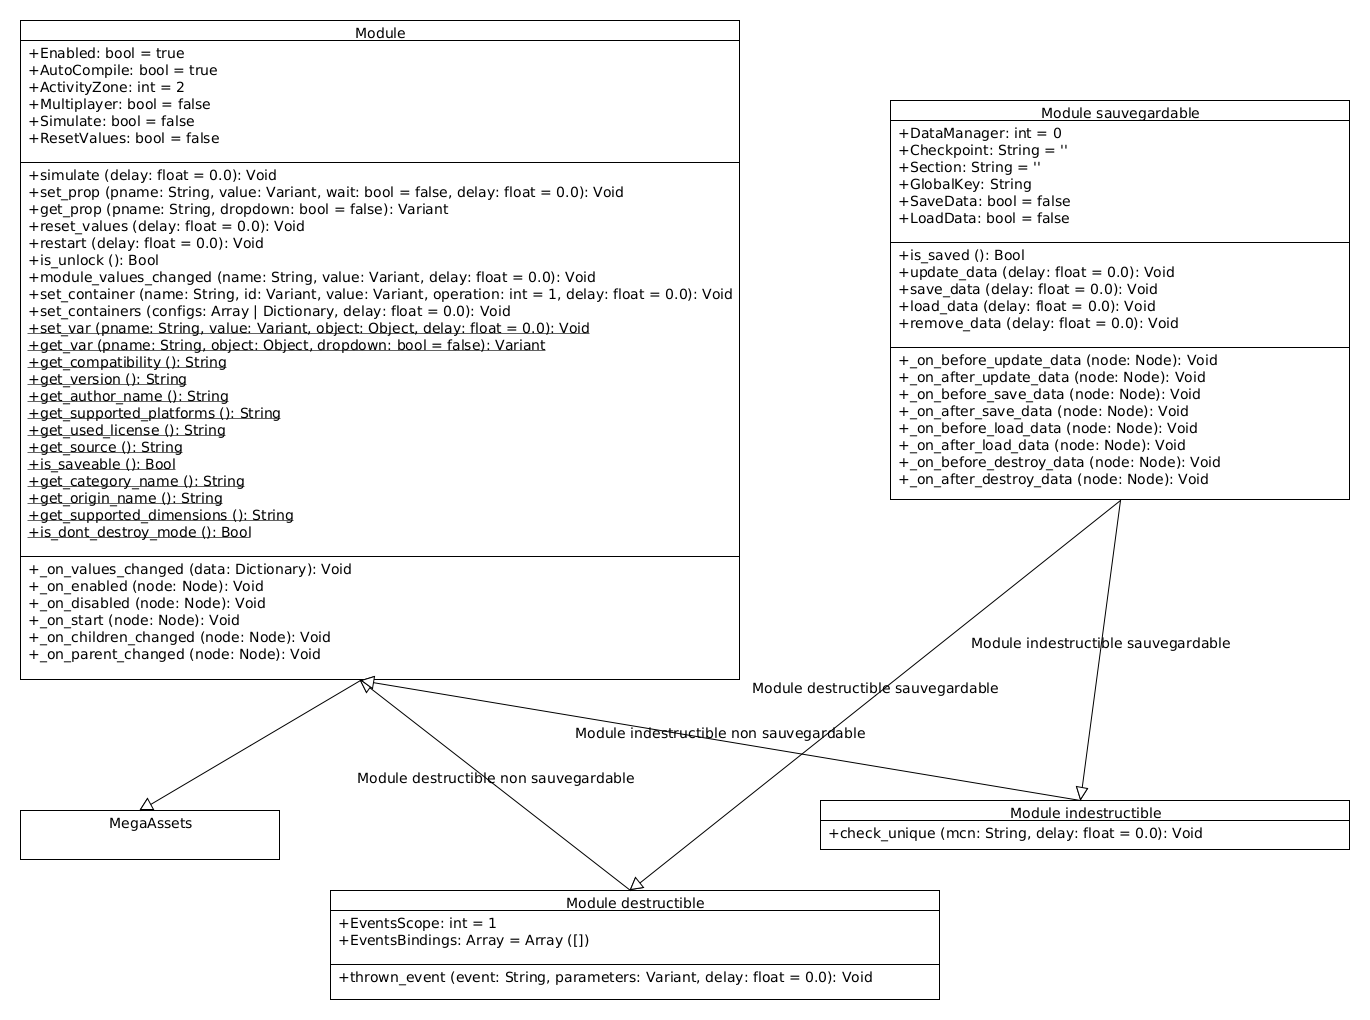
\includegraphics[width = 550pt]{basic_diagram.png}\end{center}
		\caption{Diagramme récapitulatif des fonctionnalités de base}
		\label{Diagramme récapitulatif des fonctionnalités de base}
	\end{figure}

	% Mega assets module code structure.
	\section{Structure du code d'un module}
	Tous les modules possèdent la même structure de code à savoirs:
	\begin{itemize}
		\item[+] Tout en haut avant tout code se trouve des informations à propos du module en question. 
		Bien évidement, certaines de ces informations sont récupérable via du code à travers certaines 
		fonctions offertes par le module.
		\item[+] Les attributs ou variables de classe.
		\item[+] Les signals ou événements.
		\item[+] Les variables particulières.
		\item[+] La gestion des entrées.
		\item[+] La logique et tâches principaux.
		\item[+] Les fonctionnalités disponibles.
	\end{itemize}
	\begin{description}
		\item[>> Les attributs ou variables de classe :] Partie comportant toutes les données néccessaires à 
		la bonne marche du module. Ces variables ne sont pas privées. Ainsi, le développeur a donc la 
		possibilité de pouvoir y accédées.\\
		\item[>> Les signals ou événements :] Partie regroupant tous les événements dont dispose le module.
		\\
		\item[>> Les variables particulières :] Partie comportant des données clées du module. Ces variables
		sont privées donc inaccessible aux développeurs.\\
		\item[>> La gestion des entrées :] Partie regroupant toutes les fonctions de contrôle des valeurs
		des champs du module. Cette partie joue un rôle important dans le fonctionnement du module. C'est
		elle qui est responsable des exigences du module. Son objectif est d'aider le développeur à bien
		configuré le module afin d'éviter les erreurs inutiles. Les méthodes de cette partie sont toutes
		privées.\\
		\item[>> Logique et tâches principaux :] Cette partie représente le pilier centrale du module. Elle
		traite les différentes données issues des configurations du \textit{\textcolor{gray}{GameMaster}} 
		afin de coordonner le comportement et le fonctionnement du module. C'est le coeur du module et
		toutes les méthodes de cette partie sont privées.\\
		\item[>> Les fonctionnalités disponibles :] Cette partie comporte toutes les méthodes offerte par le
		module pour son utilisation. Toutes les fonctions de cette partie sont publiques.
	\end{description}

	% Mega assets module creation.
	\section{Création d'un module}
	Cette section est uniquement dédiée aux développeurs qui souhaite créé leur propre module en utilisant
	\textcolor{gray}{\textit{Godot Mega Assets}}. Comme vous pouvez le constater, les modules de ce 
	framework suivent tous, une structure bien définie, nous permettant ainsi d'énumérer les types de base
	suivants: \textcolor{darkgreen}{Destructible, Indestructible, Saveable, Recordable} et
	\textcolor{darkgreen}{Module}.
	\begin{description}
		\item[>> \textcolor{darkgreen}{Module}:] C'est la classe de base de tous les modules. Elle hérite
		directement de la classe \textbf{\textcolor{darkgreen}{\\MegaAssets}}.\\
		\item[>> \textcolor{darkgreen}{Destructible}:] C'est la classe de base de tous les modules de nature
		destructible. Elle hérite de la classe \textcolor{darkgreen}{Module}.\\
		\item[>> \textcolor{darkgreen}{Indestructible}:] C'est la classe de base de tous les modules de
		nature indestructible. Elle hérite de la classe \textcolor{darkgreen}{Module}.\\
		\item[>> \textcolor{darkgreen}{Saveable}:] C'est la classe de base de tous les modules destructibles
		et sauvegardables. Elle hérite de la classe \textcolor{darkgreen}{Destructible}.\\
		\item[>> \textcolor{darkgreen}{Recordable}:] C'est la classe de base de tous les modules
		indestuctibles et sauvegardables. Elle hérite de la classe \textcolor{darkgreen}{Indestructible}.
	\end{description}
	Tout ce que nous venons d'évoquer peut être mis dans un schéma pour avoir une vue d'ensemble
	sur les différentes relations entre les classes de base.
	\begin{figure}[h]
		\begin{center}
			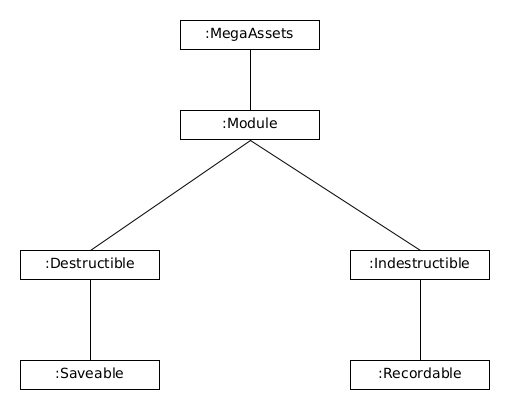
\includegraphics[width = 350pt, height = 300pt]{module_creation_structure.png}
		\end{center} \caption{Diagramme récapitulatif des relations entre les classes de base}
		\label{Diagramme récapitulatif des relations entre les classes de base}
	\end{figure}
	\\Choisissez celle que vous voulez en fonction du comportement et du fonctionnement de votre future
	module. En ce qui concerne la gestion des différentes propriétés au sein du module, des méthodes ont été
	prévues pour cela.\\
	% Void thrown_event () feature description.
	\begin{description}
		\item [+ \textcolor{red}{void} \textcolor{blue}{thrown\_event} (event, parameters, delay = 0.0):]
		Lève un événement donné. Elle prend également en charge la portée de l'événement ainsi que sa 
		liaison externe vers d'autres exécutions. Notez qu'elle n'utilise pas la fonction
		\href{https://docs.godotengine.org/en/stable/classes/class_object.html#class-object-method-emit-signal}{\textit{\textcolor{blue}{emit\_signal ()}}} dans l'émission d'événement et n'est définie que dans la 
		classe \textcolor{darkgreen}{Module}.
		\begin{itemize}
			\item [>> \textbf{\textcolor{darkgreen}{String} event}:] Quel est le nom de l'événement à
			invoqué ?
			\item [>> \textbf{\textcolor{darkgreen}{Variant} parameters}:] L'événement en question possède
			t-il des paramètres à renvoyés à ses écouteurs ?
			\item [>> \textbf{\textcolor{red}{float} delay}:] Quel est le temps mort avant le déclenchement
			de l'événement en question ?\\
		\end{itemize}
	\end{description}
	% Void module_values_event () feature description.
	\newpage \begin{description}
		\item [+ \textcolor{red}{void} \textcolor{blue}{module\_values\_changed} (name, value, delay = 
		0.0):] Lève l'événement nommé \textit{\textcolor{gray}{\\values\_changed}} avec des informations 
		permettant au écouteurs de s'informer du changement de valeur d'une propriété au sein d'un module. 
		Notez qu'elle se sert de la fonction \textit{\textcolor{blue}{thrown\_event ()}} pour accomplir son
		objectif et n'est définie que dans la classe \textcolor{darkgreen}{Module}.
		\begin{itemize}
			\item [>> \textbf{\textcolor{darkgreen}{String} name}:] Quel est le nom de la propriété dont la
			valeur à subit de(s) changement(s) ?
			\item [>> \textbf{\textcolor{darkgreen}{Variant} value}:] Quelle est la nouvelle valeur de la
			propriété référée ?
			\item [>> \textbf{\textcolor{red}{float} delay}:] Quel est le temps mort avant le déclenchement
			de l'événement en question ?\\
		\end{itemize}
	\end{description}
	% Void check_unique () feature description.
	\begin{description}
		\item [+ \textcolor{red}{void} \textcolor{blue}{check\_unique} (mcn, delay = 0.0):] Le type du
		module de nature indestructible a t-il \\plusieurs instances de lui même dans l'arbre de la scène
		définit ? Si c'est le cas, une erreur se lèvera pour notifier à l'utilisateur de l'unicité des
		modules indestructibles. Notez que cette méthode n'est définie que dans la classe
		\textcolor{darkgreen}{Indestructible}.
		\begin{itemize}
			\item [>> \textbf{\textcolor{darkgreen}{String} mcn}:] Contient le nom de la classe du module
			dont l'instance ne peut être suppérieur à 1.
			\item [>> \textbf{\textcolor{red}{float} delay}:] Quel est le temps mort avant la vérification
			de l'unicité du module en question ?\\
		\end{itemize}
	\end{description}
	% Void bind_prop () method description.
	\begin{description}
		\item [+ \textcolor{red}{void} \textcolor{blue}{bind\_prop} (...)]: Ajoute une propriété dans la
		liste des propriétés d'un script. N'appelez cette méthode que dans la fonction virtuelle:
		\href{https://docs.godotengine.org/en/stable/classes/class_object.html#class-object-method-init}
		{\textit{\textcolor{blue}{\_init ()}}}. Pour avoir plus d'informations à ce sujet, \\consulter la
		documentation sur la classe \textbf{\textcolor{darkgreen}{MegaAssets}}.\\
	\end{description}
	% Void listen_notifications () method description.
	\begin{description}
		\item [+ \textcolor{red}{void} \textcolor{blue}{listen\_notifications} (...)]: Ecoute les
		notifications de l'éditeur pour pouvoir ensuite \\déclenché les configurations éffectuées à propos 
		de la clé \textit{\textcolor{gray}{notification}} sur les variables d'un script. Pour avoir plus
		d'informations à ce sujet, consulter la documentation sur la classe \textbf{\textcolor{darkgreen}
		{MegaAssets}}.\\
	\end{description}
	% Void reset_props_value () method description.
	\begin{description}
		\item [+ \textcolor{red}{void} \textcolor{blue}{reset\_props\_value} (...)]: Rénitialise la valeur 
		d'un ou de plusieurs propriétés d'un script. Pour avoir plus d'informations à ce sujet, consulter la
		documentation sur la classe \textbf{\textcolor{darkgreen}{MegaAssets}}.\\
	\end{description}
	% Array get_properties () method description.
	\begin{description}
		\item [+ \textcolor{darkgreen}{Array} \textcolor{blue}{get\_properties} (...)]: Renvoie la liste de 
		toutes les propriétés définient au sein du \\dictionaire \textit{\textcolor {gray}{\_\_props\_\_}}.
		Pour avoir plus d'informations à ce sujet, consulter la documentation sur la classe
		\textbf{\textcolor{darkgreen}{MegaAssets}}.\\
	\end{description}
	% Void destroy_props () method description.
	\begin{description}
		\item [+ \textcolor{red}{void} \textcolor{blue}{destroy\_props} (...)]: Détruit un ou plusieurs
		propriété(s) associée(s) à un script. Pour avoir plus d'informations à ce sujet, consulter la
		documentation sur la classe \textbf{\textcolor{darkgreen}{MegaAssets}}.\\
	\end{description}
	% Void override_prop () method description.
	\begin{description}
		\item [+ \textcolor{red}{void} \textcolor{blue}{override\_prop} (...)]: Redéfinit une propriété
		donnée. Pour avoir plus d'informations à ce \\sujet, consulter la documentation sur la classe
		\textbf{\textcolor{darkgreen}{MegaAssets}}.\\
	\end{description}

	% Mega assets destructible module creation template.
	\newpage \section{Template: Création d'un module destructible}
	\textbf{Code: GDScript}
	\begin{lstlisting}
		# Dependencies.
		tool class_name YourModuleType extends Destructible;

		# Contains all module properties.
		func _create_module_properties () -> void:
			# Declare all module variables here with "bind_prop ()" method.
			pass;

		# This method is called on game initialization and before all nodes instanciation.
		func _init (): self._create_module_properties ();

		# What is the type of your module ?
		func get_class () -> String: return "YourModuleType";

		# What is the current version of your module ?
		static func get_version () -> String: return "1.0.0";

		# What is the supported dimensions of your module ? (Optional).
		static func get_supported_dimensions () -> String: return "2D || 3D";

		# What is the category of your module ? (Optional).
		static func get_category_name () -> String: return "YourModuleCategoryName";
		
		# What is the supported platforms of your module ? (Optional).
		static func get_supported_platforms () -> String: return "ANDROID || MACOSX || WINDOWS || LINUX";

		# Do you want to allow on others users to restart your module ? (Optional).
		func restart (_delay: float = 0.0) -> void: if self.is_unlock (): pass;

		# Do you want to give an overview of the main operation of your module ? Called when you pressed on "Simulate" module property. (Optional if you destroy "Simulate" property with .destroy_props () method).
		func simulate (_delay: float = 0.0) -> void: if self.is_unlock (): pass;
	\end{lstlisting}

	% Mega assets indestructible module creation template.
	\newpage \section{Template: Création d'un module indestructible}
	\textbf{Code: GDScript}
	\begin{lstlisting}
		# Dependencies.
		tool class_name YourModuleType extends Indestructible;

		# Contains all module properties.
		func _create_module_properties () -> void:
			# Declare all module variables here with "bind_prop ()" method.
			pass;

		# This method is called on game initialization and before all nodes instanciation.
		func _init (): self._create_module_properties ();

		# Called before ready method run.
		func _enter_tree (): self.check_unique (self.get_class ());

		# What is the type of your module ?
		func get_class () -> String: return "YourModuleType";

		# What is the current version of your module ?
		static func get_version () -> String: return "1.0.0";

		# What is the supported dimensions of your module ? (Optional).
		static func get_supported_dimensions () -> String: return "2D || 3D";

		# What is the category of your module ? (Optional).
		static func get_category_name () -> String: return "YourModuleCategoryName";
		
		# What is the supported platforms of your module ? (Optional).
		static func get_supported_platforms () -> String: return "ANDROID || MACOSX || WINDOWS || LINUX";

		# Do you want to allow on others users to restart your module ? (Optional).
		func restart (_delay: float = 0.0) -> void: if self.is_unlock (): pass;

		# Do you want to give an overview of the main operation of your module ? Called when you pressed on "Simulate" module property. (Optional if you destroy "Simulate" property with .destroy_props () method).
		func simulate (_delay: float = 0.0) -> void: if self.is_unlock (): pass;
	\end{lstlisting}
\end{document}